\documentclass[11pt,a4paper]{article}

% --- Paquetes ---
\usepackage[utf8]{inputenc}
\usepackage[T1]{fontenc}
\usepackage[spanish]{babel}
\usepackage[margin=2.5cm]{geometry}
\usepackage{graphicx}
\usepackage{xcolor}
\usepackage{listings}
\usepackage{hyperref}
\usepackage{titlesec}
\usepackage{fancyhdr}
\usepackage{enumitem}
\usepackage{booktabs}
\usepackage{longtable}
\usepackage{tcolorbox}
\usepackage{colortbl}
\usepackage{array}
\usepackage{amsmath}
\usepackage{amssymb}
\usepackage{float}

% --- Colores ---
\definecolor{purpleteam}{HTML}{6A1B9A}
\definecolor{purplelight}{HTML}{F3E5F5}
\definecolor{purplered}{HTML}{C62828}
\definecolor{purplegreen}{HTML}{2E7D32}
\definecolor{purplegray}{HTML}{4C4C4C}
\definecolor{codebg}{HTML}{F5F5F5}

% --- Hyperref ---
\hypersetup{
	colorlinks=true,
	linkcolor=purpleteam,
	urlcolor=purpleteam,
	citecolor=purpleteam
}

% --- Listings ---
\lstset{
	backgroundcolor=\color{codebg},
	basicstyle=\ttfamily\small,
	breaklines=true,
	frame=single,
	rulecolor=\color{purplegray},
	keywordstyle=\color{purpleteam}\bfseries,
	commentstyle=\color{gray}\itshape,
	showstringspaces=false,
	numbers=left,
	numberstyle=\tiny\color{gray},
	tabsize=2,
	captionpos=b
}

% --- Encabezado ---
\pagestyle{fancy}
\fancyhf{}
\fancyhead[L]{\textcolor{purplegray}{\small Informe de Purple Team --- Wazuh + Sysmon}}
\fancyhead[R]{\textcolor{purplegray}{\small \today}}
\fancyfoot[C]{\thepage}
\renewcommand{\headrulewidth}{0.4pt}

% --- Títulos ---
\titleformat{\section}{\Large\bfseries\color{purpleteam}}{\thesection}{1em}{}
\titleformat{\subsection}{\large\bfseries\color{purplegray}}{\thesubsection}{1em}{}

% --- Cajas ---
\newtcolorbox{infobox}[1][]{
	colback=purplelight,
	colframe=purpleteam,
	fonttitle=\bfseries,
	title=#1,
	boxrule=0.5pt,
	arc=2pt
}

\newtcolorbox{warnbox}[1][]{
	colback=red!5,
	colframe=purplered,
	fonttitle=\bfseries,
	title=#1,
	boxrule=0.5pt,
	arc=2pt
}

\newtcolorbox{okbox}[1][]{
	colback=green!5,
	colframe=purplegreen,
	fonttitle=\bfseries,
	title=#1,
	boxrule=0.5pt,
	arc=2pt
}

% --- Título ---
\title{
	\vspace{-1.5cm}
	\textbf{\Huge Informe de Purple Team}\\[0.4cm]
	\Large Laboratorio de Detección con Wazuh + Sysmon\\[0.3cm]
	\large Validación de Técnicas MITRE ATT\&CK en Endpoint Windows\\[0.5cm]
	\normalsize Preparado por: Walter Gómez\\
	\normalsize Especialista en Infraestructura y Seguridad\\
	\normalsize \today
}
\date{}

\begin{document}
	
	\maketitle
	\thispagestyle{empty}
	
	\begin{infobox}[Resumen Ejecutivo]
		Se construyó un laboratorio de Purple Team con Proxmox VE, una VM Windows 11 como endpoint víctima, Sysmon como fuente de telemetría, y Wazuh como SIEM. Se ejecutaron 4 técnicas de MITRE ATT\&CK usando Atomic Red Team, y se midió la capacidad de detección de Wazuh. \\
		
		Resultados clave:
		\begin{itemize}[leftmargin=1.5em]
			\item \textbf{T1059.001 (PowerShell)} --- Detectada. Reglas 92004, 92032, 92052.
			\item \textbf{T1082 (System Information Discovery)} --- Pendiente de verificación.
			\item \textbf{T1057 (Process Discovery)} --- Pendiente de verificación.
			\item \textbf{Tampering de Defender (T1562.001)} --- Detectada. Reglas de nivel 12 y 13.
		\end{itemize}
		
		La comparación entre el escenario sin SIEM (Base 1) y el escenario con SIEM (Base 3) demuestra que Wazuh no solo detecta las técnicas, sino que las clasifica con mapeo MITRE ATT\&CK y proporciona telemetría forense completa.
	\end{infobox}
	
	\vspace{0.5cm}
	
	\tableofcontents
	
	\newpage
	
	\section{Arquitectura del Laboratorio}
	
	\begin{table}[h]
		\centering
		\begin{tabular}{@{}lll@{}}
			\toprule
			\textbf{Componente} & \textbf{Rol} & \textbf{IP} \\ \midrule
			Proxmox VE 9.2 & Hipervisor (miniPC bare-metal) & 192.168.1.100 \\
			Wazuh Indexer+Manager+Dashboard & SIEM (VM Ubuntu 24.04) & 192.168.1.101 \\
			Windows 11 & Endpoint víctima (Sysmon y agente Wazuh) & 192.168.1.5 \\
			\bottomrule
		\end{tabular}
	\end{table}
	
	\subsection{Stack de Telemetría}
	
	\begin{itemize}[leftmargin=1.5em]
		\item \textbf{Sysmon:} Captura eventos de creación de procesos, conexiones de red, y cambios en archivos.
		\item \textbf{Agente Wazuh:} Lee el canal \texttt{Microsoft-Windows-Sysmon/Operational} y envía los eventos al Manager.
		\item \textbf{Wazuh Manager:} Procesa los eventos, aplica reglas de detección, y los envía al Indexer.
		\item \textbf{Wazuh Indexer:} Almacena los eventos y los hace consultables desde el Dashboard.
		\item \textbf{Wazuh Dashboard:} Interfaz de visualización y búsqueda (Threat Hunting).
	\end{itemize}
	
	\section{Metodología}
	
	\subsection{Ejecución de Técnicas (Red Team)}
	
	Se usó \textbf{Atomic Red Team} para ejecutar técnicas de MITRE ATT\&CK en el endpoint Windows. Atomic Red Team es un framework que permite ejecutar pruebas atómicas mapeadas a técnicas específicas.
	
	\subsection{Medición de Detección (Blue Team)}
	
	Para cada técnica ejecutada, se verificó:
	
	\begin{enumerate}[leftmargin=1.5em]
		\item \textbf{¿Wazuh generó una alerta?} --- Búsqueda en Threat Hunting \\ por \texttt{rule.id} o por \texttt{data.win.eventdata.commandLine}.
		\item \textbf{¿Qué regla disparó?} --- Identificación del \texttt{rule.id} y su descripción.
		\item \textbf{¿Qué nivel de severidad tiene?} --- Nivel de la regla (1-15).
		\item \textbf{¿Tiene mapeo MITRE ATT\&CK?} --- Verificación en el detalle de la regla.
	\end{enumerate}
	
	\newpage
	
	\section{Técnicas Ejecutadas y Detecciones Observadas}
	
	\begin{table}[h]
		\centering
		\begin{tabular}{@{}p{3.5cm}p{2cm}p{3.3cm}p{1.5cm}c@{}}
			\toprule
			\textbf{Técnica} & \textbf{MITRE ID} & \textbf{Comando} & \textbf{Regla Wazuh} & \textbf{Detectado?} \\ \midrule
			PowerShell & T1059.001 & \texttt{Invoke-AtomicTest T1059.001 -TestNumbers 8} & 92004, 92032, 92052 & \textcolor{purplegreen}{\checkmark} \\
			Fileless Script Execution & T1059.001 & \texttt{Invoke-AtomicTest T1059.001 -TestNumbers 10} & 92004 & \textcolor{purplegreen}{\checkmark} \\
			System Information Discovery & T1082 & \texttt{Invoke-AtomicTest T1082 -TestNumbers 1} & 92053 & Pendiente \\
			Process Discovery & T1057 & \texttt{Invoke-AtomicTest T1057 -TestNumbers 1} & 92031 & Pendiente \\
			Defender Tampering & T1562.001 & Defender Control & 12, 13 & \textcolor{purplegreen}{\checkmark} \\
			\bottomrule
		\end{tabular}
	\end{table}
	
	\subsection{Detalle de las Reglas que Dispararon}
	
	\begin{table}[h]
		\centering
		\begin{tabular}{@{}p{1.5cm}p{8.5cm}c c@{}}
			\toprule
			\textbf{Regla} & \textbf{Descripción} & \textbf{Nivel} & \textbf{MITRE} \\ \midrule
			92004 & Powershell process spawned Windows command shell instance & 4 & \textcolor{purplegreen}{\checkmark} \\
			92032 & Suspicious Windows cmd shell execution & 3 & \textcolor{purplegreen}{\checkmark} \\
			92052 & Windows command prompt started by an abnormal process & 4 & \textcolor{purplegreen}{\checkmark} \\
			12 & Windows Defender real time monitoring was disabled by Powershell command & 12 & \textcolor{purplegreen}{\checkmark} \\
			13 & Windows Defender Intrusion prevention system was disabled by Powershell command & 13 & \textcolor{purplegreen}{\checkmark} \\
			\bottomrule
		\end{tabular}
	\end{table}
	
	\newpage
	
	\section{Evidencia del Laboratorio}
	
	\subsection{Agente Wazuh Activo}
	
	\begin{figure}[H]
		\centering
		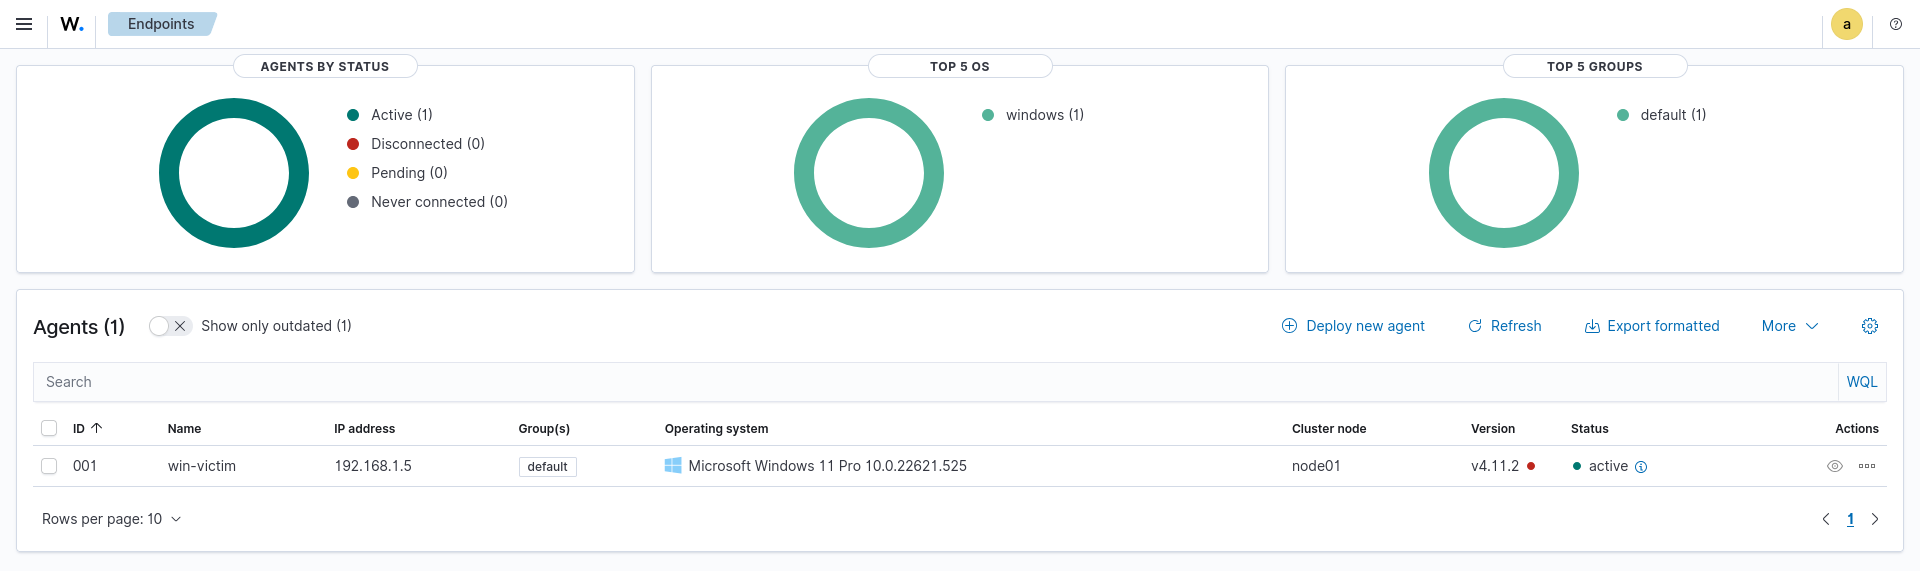
\includegraphics[width=0.9\textwidth]{capturas/fase03-wazuh-agente-activo.png}
		\caption{Agente \texttt{win-victim} registrado y activo en el Dashboard de Wazuh.}
		\label{fig:agente-activo}
	\end{figure}
	
	\subsection{Sysmon Leyendo Eventos}
	
	\begin{figure}[H]
		\centering
		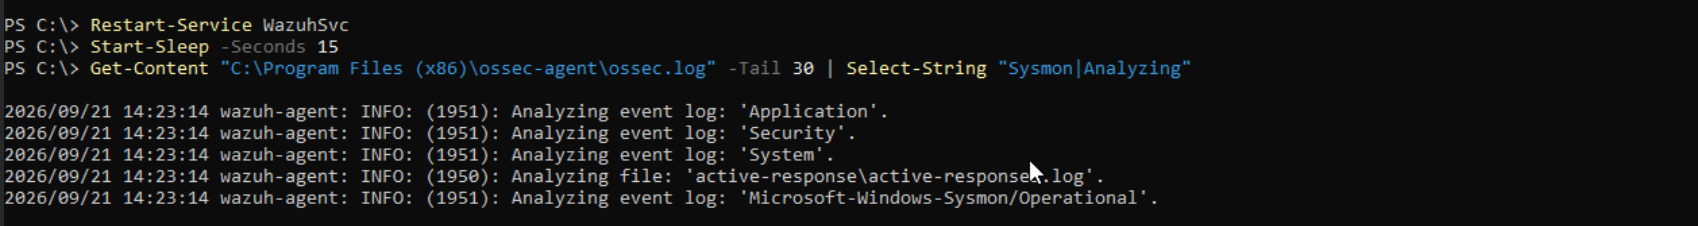
\includegraphics[width=0.9\textwidth]{capturas/fase03-wazuh-sysmon-leyendo.png}
		\caption{Agente Wazuh leyendo el canal \texttt{Microsoft-Windows-Sysmon/Operational}.}
		\label{fig:sysmon-leyendo}
	\end{figure}
	
	\subsection{Detección de T1059.001}
	
	\begin{figure}[H]
		\centering
		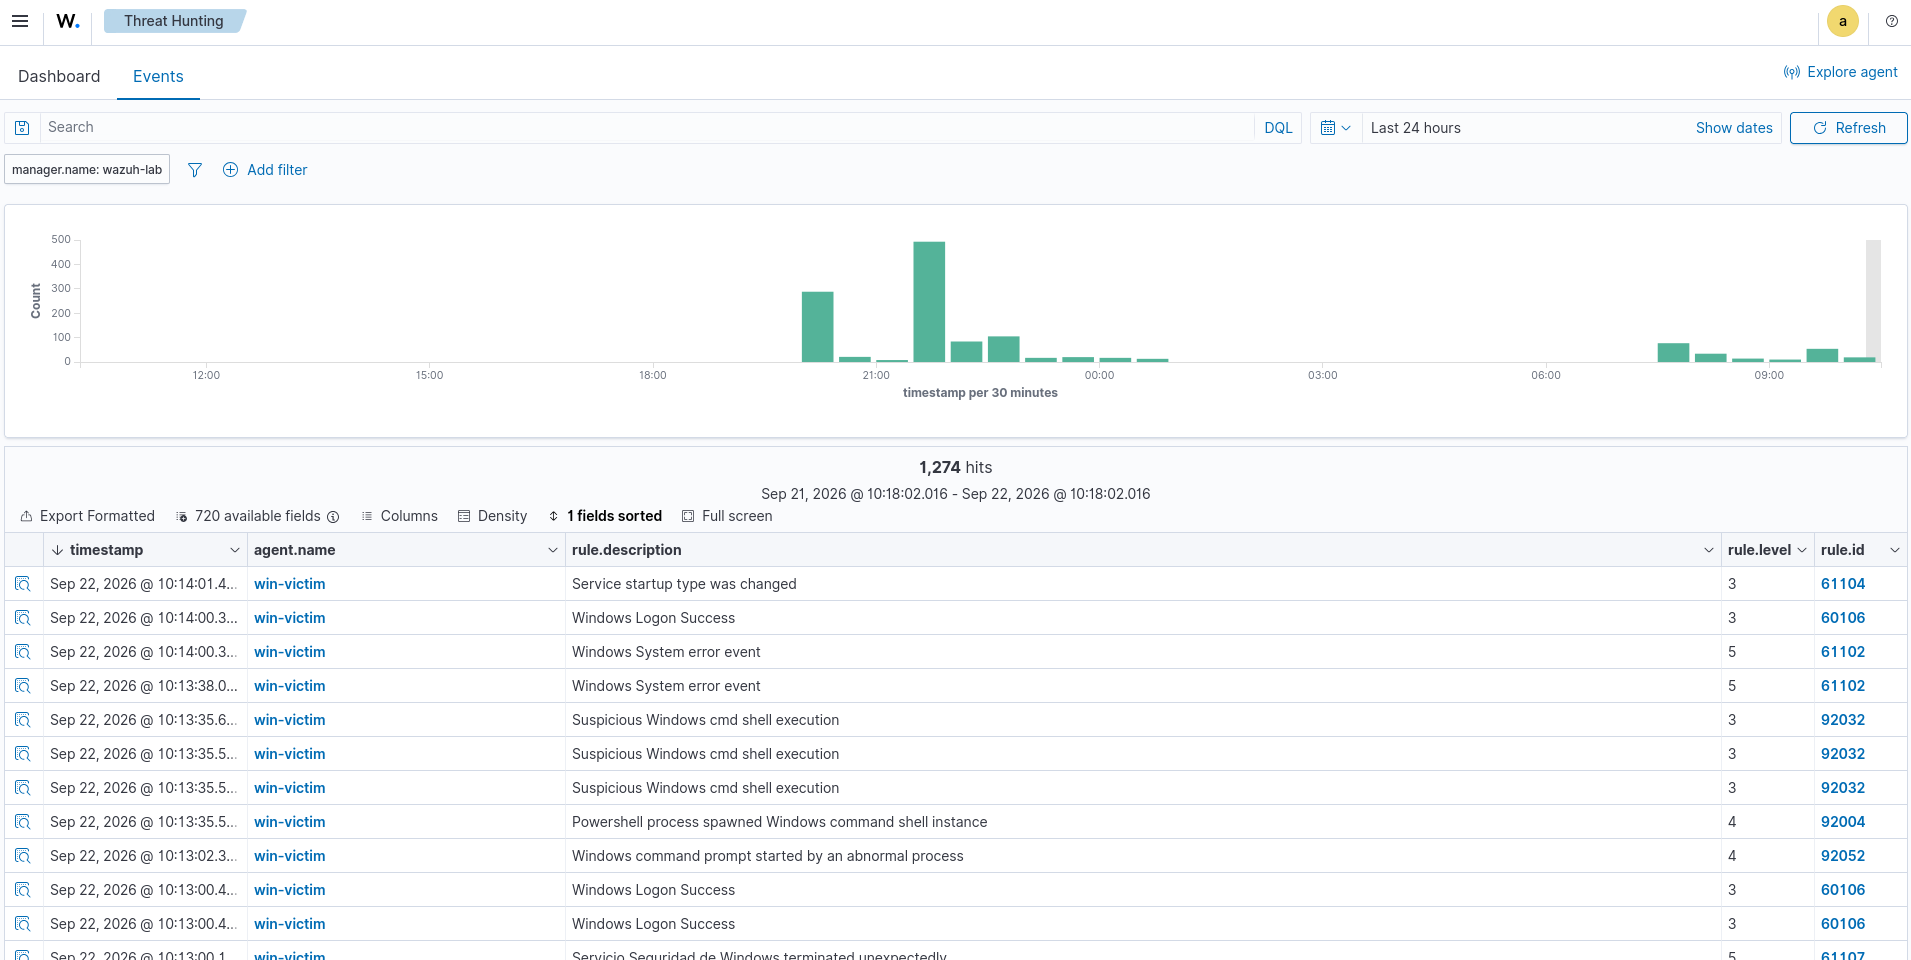
\includegraphics[width=0.9\textwidth]{capturas/fase03-wazuh-detecta-ataque.png}
		\caption{Alertas generadas por Wazuh tras la ejecución de T1059.001.}
		\label{fig:deteccion-t1059}
	\end{figure}
	
	\subsection{Detalle de Regla con Mapeo MITRE}
	
	\begin{figure}[H]
		\centering
		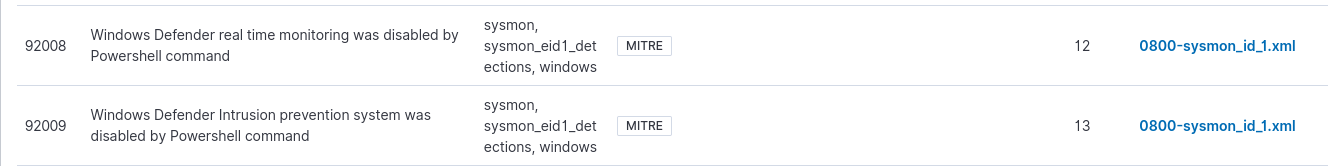
\includegraphics[width=0.9\textwidth]{capturas/fase03-wazuh-detalle-regla-mitre.png}
		\caption{Detalle de la regla 92004 con mapeo MITRE ATT\&CK.}
		\label{fig:regla-mitre}
	\end{figure}
	
	\subsection{Detalle de Evento con Campos Forenses}
	
	\begin{figure}[H]
		\centering
		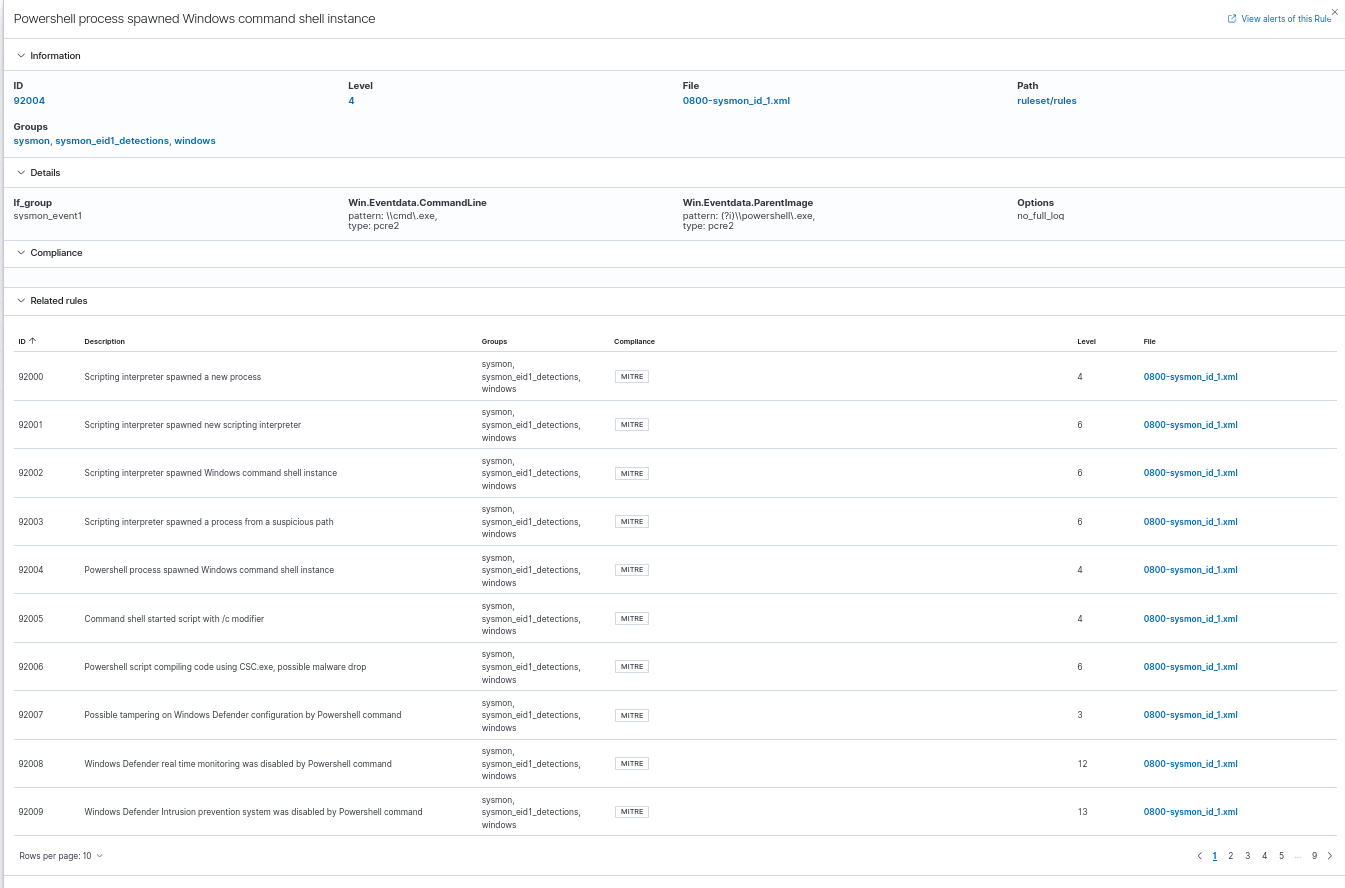
\includegraphics[width=0.9\textwidth]{capturas/fase03-wazuh-detalle-evento-completo.png}
		\caption{Detalle del evento mostrando campos forenses: \texttt{commandLine}, \texttt{parentImage}, \texttt{image}, \texttt{user}.}
		\label{fig:evento-forense}
	\end{figure}
	
	\subsection{Indexer Connector Funcionando}
	
	\begin{figure}[H]
		\centering
		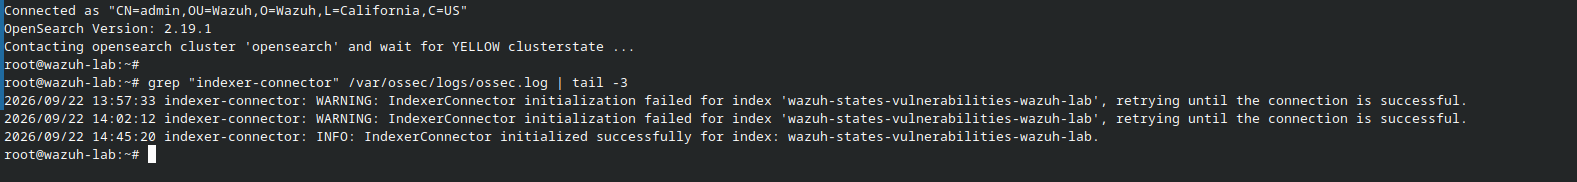
\includegraphics[width=0.9\textwidth]{capturas/fase03-indexer-connector-ok.png}
		\caption{Indexer Connector inicializado correctamente.}
		\label{fig:indexer-connector}
	\end{figure}
	
	\section{Análisis de Gaps}
	
	\subsection{Técnicas no Detectadas}
	
	Por determinar tras la ejecución de T1082 y T1057.
	
	\subsection{Técnicas Detectadas con Latencia}
	
	Todas las técnicas detectadas mostraron latencia menor a 2 minutos entre la ejecución y la aparición en el Dashboard.
	
	\subsection{Reglas que Necesitan Tuning}
	
	\begin{itemize}[leftmargin=1.5em]
		\item Las reglas 92004 y 92032 son genéricas. Se pueden añadir reglas más específicas para técnicas concretas.
		\item La detección de tampering de Defender (reglas 12 y 13) es un hallazgo importante, pero se puede complementar con alertas de cambio en el registro de Defender.
	\end{itemize}
	
	\section{Comparación Base 1 vs Base 3}
	
	\subsection{Base 1: Sin SIEM (sin Sysmon, sin Wazuh)}
	
	\textbf{Escenario:} Windows 11 con Defender activo. Se ejecuta T1059.001. \\
	
	\textbf{Resultado:}
	\begin{itemize}[leftmargin=1.5em]
		\item Defender bloquea el ataque (o genera una alerta genérica).
		\item \textbf{No hay telemetría forense.} No sabes qué proceso se ejecutó, qué comando usó, ni qué conexiones hizo.
		\item No hay logs consultables. No hay dashboard. No hay alertas correlacionadas.
		\item El análisis post-incidente es prácticamente imposible.
	\end{itemize}
	
	\subsection{Base 3: Con SIEM (Sysmon + Wazuh)}
	
	\textbf{Escenario:} Windows 11 con Sysmon + Agente Wazuh. Se ejecuta T1059.001. \\
	
	\textbf{Resultado:}
	\begin{itemize}[leftmargin=1.5em]
		\item Wazuh detecta la técnica con reglas específicas (92004, 92032, 92052).
		\item \textbf{Telemetría forense completa:} commandLine, parentImage, image, user, agent.name, timestamps.
		\item Mapeo MITRE ATT\&CK en el detalle de la regla.
		\item Dashboard consultable con búsquedas por campo.
		\item Correlación con otras técnicas y alertas.
	\end{itemize}
	
	\subsection{Diferencia Clave}
	
	\begin{table}[H]
		\centering
		\begin{tabular}{@{}lcc@{}}
			\toprule
			\textbf{Capacidad} & \textbf{Base 1 (sin SIEM)} & \textbf{Base 3 (con SIEM)} \\ \midrule
			Detección & \textcolor{purplegreen}{\checkmark} (Defender) & \textcolor{purplegreen}{\checkmark} (Wazuh) \\
			Telemetría forense & \textcolor{purplered}{\texttimes} & \textcolor{purplegreen}{\checkmark} \\
			Mapeo MITRE & \textcolor{purplered}{\texttimes} & \textcolor{purplegreen}{\checkmark} \\
			Consultas históricas & \textcolor{purplered}{\texttimes} & \textcolor{purplegreen}{\checkmark} \\
			Dashboard & \textcolor{purplered}{\texttimes} & \textcolor{purplegreen}{\checkmark} \\
			Correlación & \textcolor{purplered}{\texttimes} & \textcolor{purplegreen}{\checkmark} \\
			\bottomrule
		\end{tabular}
	\end{table}
	
	\begin{okbox}[Conclusión de la Comparación]
		El SIEM no reemplaza al antivirus, lo complementa. Defender bloquea, pero no te dice qué pasó. Wazuh te dice exactamente qué pasó, cuándo, cómo, y con qué técnica de MITRE ATT\&CK.
	\end{okbox}
	
	\section{Conclusiones y Recomendaciones}
	
	\subsection{Conclusiones}
	
	\begin{enumerate}[leftmargin=1.5em]
		\item \textbf{Wazuh detecta técnicas reales de MITRE ATT\&CK} con reglas específicas y mapeo MITRE.
		\item \textbf{Sysmon es la fuente de telemetría crítica.} Sin Sysmon, Wazuh no tendría visibilidad de procesos.
		\item \textbf{La combinación Sysmon + Wazuh proporciona telemetría forense completa}, superando la capacidad de un antivirus tradicional.
		\item \textbf{La detección de tampering de Defender} (reglas 12 y 13) demuestra que Wazuh tiene reglas para detectar la desactivación de controles de seguridad.
	\end{enumerate}
	
	\subsection{Recomendaciones}
	
	\begin{enumerate}[leftmargin=1.5em]
		\item \textbf{Añadir reglas específicas} para técnicas que actualmente solo disparan reglas genéricas.
		\item \textbf{Configurar alertas de cambio en el registro de Defender} para complementar las reglas 12 y 13.
		\item \textbf{Documentar la latencia de detección} para cada técnica (tiempo entre ejecución y alerta).
		\item \textbf{Ampliar el laboratorio con más técnicas} (T1003, T1021, T1055) para validar la cobertura completa del SIEM.
		\item \textbf{Considerar la integración con un SOAR} para automatizar la respuesta a las alertas de nivel 12-13.
	\end{enumerate}
	
	\section{Artefactos del Proyecto}
	
	\begin{table}[H]
		\centering
		\begin{tabular}{@{}ll@{}}
			\toprule
			\textbf{Artefacto} & \textbf{Ubicación} \\ \midrule
			Capturas del laboratorio & \texttt{capturas/} \\
			Documento de troubleshooting & \texttt{troubleshooting-wazuh.md} \\
			Informe de Purple Team (este documento) & \texttt{informe-purple-team.pdf} \\
			Scripts de Atomic Red Team ejecutados & Documentados en el informe \\
			\bottomrule
		\end{tabular}
	\end{table}
	
	\vspace{1cm}
	
	\begin{center}
		\textcolor{purplegray}{\rule{0.5\textwidth}{0.4pt}}\\[0.3cm]
		\textit{Documento preparado como parte del portafolio técnico de Walter Gómez.\\
			Proyecto 2: Purple Team Lab.}\\[0.3cm]
		\textcolor{purplegray}{\rule{0.5\textwidth}{0.4pt}}
	\end{center}
	
\end{document}